\subsection{Performance do Quantizador}

\begin{frame}[allowframebreaks]
  \frametitle{Performance do Quantizador}
  Seja $p(x)$ a pdf do sinal de entrada $x$, então o erro médio quadrático (MSE) 
  devido à quantização será dado por
  \begin{equation} \label{eq-sqnr-quants}
  \sigma_q^2 = \sum_{k=1}^{M} \int_{t_{k-1}}^{t_k} (x - y_k)^2 p(x) \mathrm{d}x.
  \end{equation}

  Se $M$ for grande e a pdf $p(x)$ for suave, poderemos aproximar $p(x)$ no intervalo $(t_{k-1},t_{k}]$ como
  \begin{equation}
  p(x) \approx p\left(\frac{t_{k-1}+t_{k}}{2}\right) , \quad t_{k-1} < x \leq t_k ,
  \end{equation}
  e assim, a equação \ref{eq-sqnr-quants} poderá ser reescrita como
  \begin{equation} \label{eq-sqnr-quants2}
  \sigma_q^2 = \sum_{k=1}^{M} p\left(\frac{t_{k-1}+t_{k}}{2}\right) \int_{t_{k-1}}^{t_k} (x - y_k)^2 \mathrm{d}x.
  \end{equation}

  Mostra-se que
  \begin{equation} \label{eq-sqnr-int}
  \int_{t_{k-1}}^{t_k} (x - y_k)^2 \mathrm{d}x = \Delta_k \left[ \left( y_k - \frac{t_{k-1} + t_{k}}{2} \right)^2 + \frac{\Delta_k^2}{12} \right] ,
  \end{equation}
  onde $\Delta_k = t_k - t_{k-1}$ é o tamanho do passo do quantizador.

  Para minimizar o MSE devemos escolher $y_k = (t_{k-1} + t_{k})/2$, 
  de forma que o primeiro termo em \ref{eq-sqnr-int} se anule. Ou seja,
  devemos escolher os pontos de representação como o ponto médio dos limiares dos intervalos.
  (obs.: Isto ocorre devido à aproximação feita para $p$ suave e $M$ grande. No caso geral,
  deveremos ter os pontos de representação no valor esperado de cada intervalo)

  Vamos definir $p_k$ como a probabilidade de $x$ pertencer ao intervalo $(t_{k-1},t_k]$.
  Usando a aproximação feita anteriormente, teremos
  \begin{equation} \label{eq-pk-aprox}
  p_k = \Pr(t_{k-1} < x \leq t_k) \approx p\left(\frac{t_{k-1}+t_{k}}{2}\right) \Delta_k ,
  \end{equation}
  e assim podemos reescrever a equação \ref{eq-sqnr-quants2} como
  \begin{equation} \label{eq-sqnr-quants3}
  \sigma_q^2 = \frac{1}{12} \sum_{k=1}^{M} p_k \Delta_k^2 .
  \end{equation}

\end{frame}


\subsection{Quantizador Uniforme}
\begin{frame}[allowframebreaks]
  \frametitle{Performance do Quantizador Uniforme} 

  Para o quantizador uniforme o passo é constante ($\Delta_k = \Delta$ para todo $k$). Teremos assim
  \begin{equation} \label{eq-sqnr-quants-uni}
  \sigma_q^2 = \frac{\Delta^2}{12} \underbrace{ \sum_{k=1}^{M} p_k }_{=1} = \frac{\Delta^2}{12} .
  \end{equation}
  Note que a potência do ruído de quantização é independente da distribuição do sinal.

  A performance do quantizador será expressa pela relação sinal-ruído de quantização (SQNR),
  \begin{equation} \label{eq-sqnr-unif}
  \textmd{SQNR} = 10 \log \left( \frac{\sigma_x^2}{\sigma_q^2} \right) = 10 \log \left( \frac{12 \sigma_x^2}{\Delta^2} \right) \mathrm{dB}.
  \end{equation}
\end{frame}

\begin{frame}[allowframebreaks]
  \frametitle{Performance do Quantizador Uniforme - Sinal Senoidal}
  Vamos supor que o sinal de entrada seja da forma $A \sin \omega t$ e 
  um quantizador uniforme com $n$ bits ($2^n = M$). Podemos escolher $\Delta$
  para que não ocorra saturação. Faremos então $\Delta = A/2^{n-1}$.
  A potência do sinal senoidal é $\sigma_x^2 = A^2/2$. Usando agora a Equação \ref{eq-sqnr-unif}, teremos
  \begin{equation} \label{eq-sqnr-unif-sin}
  \textmd{SQNR (senoide)}  = 6n + 1.76 \mathrm{dB}.
  \end{equation}
\end{frame}

\begin{frame}[allowframebreaks]
  \frametitle{Performance do Quantizador Uniforme - Sinal Gaussiano}
  Iremos supor agora um sinal de entrada com distribuição gaussiana: $p(x)=1/\sqrt{2\pi\sigma} e^{-(x^2/2\sigma^2)}$.
  Para que a distorção por saturação seja desprezível, iremos fazer $2^{n-1} \Delta = 4 \sigma$, ou seja, teremos $\Delta = \sigma/2^{n-3}$.
  A potência média quadrática do sinal de entrada é $\sigma_x^2 = \sigma^2$. Usando agora a Equação \ref{eq-sqnr-unif}, teremos
  \begin{equation} \label{eq-sqnr-unif-gaus}
  \textmd{SQNR (gauss)}  = 6n - 7.3 \mathrm{dB}.
  \end{equation}
\end{frame}


\subsection{Quantizador Não Uniforme}
\begin{frame}%[allowframebreaks]
  \frametitle{Quantizador Não Uniforme}

  Os sinais de fala, por exemplo, estão geralmente concentrados em torno da origem.
  Desta forma, seria interessante propor um quantizador em que os passos de quantização
  fossem menores na região de menor amplitude do sinal e maiores na região de maior amplitude.
  Isto levaria a uma redução do ruído de quantização total.

  \begin{figure}[h!]
  \centering
  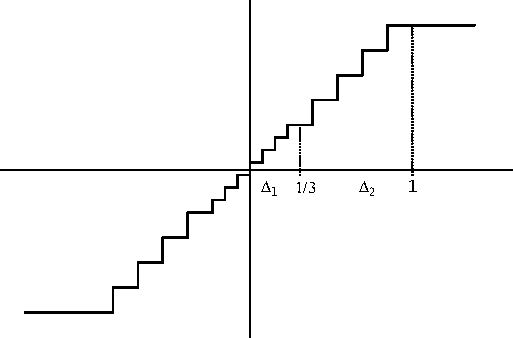
\includegraphics[width=0.4\textwidth]{images/nuquantz.pdf}
  \caption{Exemplo de quantizador não uniforme de 4 bits, com $\Delta_1 = \Delta_2/2$ \citep{tokunbo}.}
  \label{fig:nuquantz}
  \end{figure}
\end{frame}

